% !TeX spellcheck = es_ANY
\documentclass{beamer}
\usepackage[utf8]{inputenc}
\usetheme{Madrid}
\usecolortheme{beaver}
\usepackage{physics}
\usepackage{xcolor}
\usepackage[style=authortitle, backend=bibtex]{biblatex}
\addbibresource{bib/mybib}

\renewcommand*{\bibfont}{\tiny}

\newcommand\blfootnote[1]{%
  \begingroup
  \renewcommand\thefootnote{}\footnote{#1}%
  \addtocounter{footnote}{-1}%
  \endgroup
}


\makeatletter
\def\mathcolor#1#{\@mathcolor{#1}}
\def\@mathcolor#1#2#3{%
  \protect\leavevmode
  \begingroup
    \color#1{#2}#3%
  \endgroup
}

\renewcommand{\arraystretch}{2}

\title[Mauscope] %optional
{Diseño y construcción de un stage de translación en $x$, $y$ y $z$ automatizado}
 
\author[J. Barbosa] % (optional, for multiple authors)
{J. Barbosa\inst{1}}
 
\institute[] % (optional)
{
  \inst{1}%
  Departamento de Física\\
  Universidad de los Andes
}
 
\date[Diciembre 2017] % (optional)
{Sustentaci\'on, Diciembre 2017}

\setbeamerfont{footnote}{size=\tiny}

\titlegraphic{
\includegraphics[height=2cm]{figures/FacultadCiencias.pdf}}

\begin{document}
    \frame{\titlepage}
    
    \begin{frame}{Contenido}
        \tableofcontents
    \end{frame}
    
    \section{Introducción}
    \begin{frame}
        \frametitle{Introducción}
         \begin{figure}
            \centering
            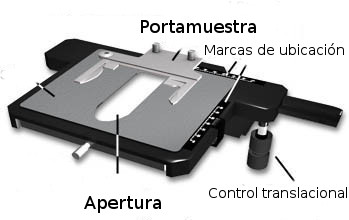
\includegraphics[width=0.5\linewidth]{figures/stage1.jpg}
        \end{figure}
        
        \begin{columns}
            \column{0.45\textwidth}
                Construcción.
            \column{0.45\textwidth}
                Automatización.
        \end{columns}
        \blfootnote{\cite{Abramowitz2015}}
    \end{frame}
    
    \begin{frame}
   		\begin{figure}[h]
   			\centering
   			\begin{tabular}{ccc}
   				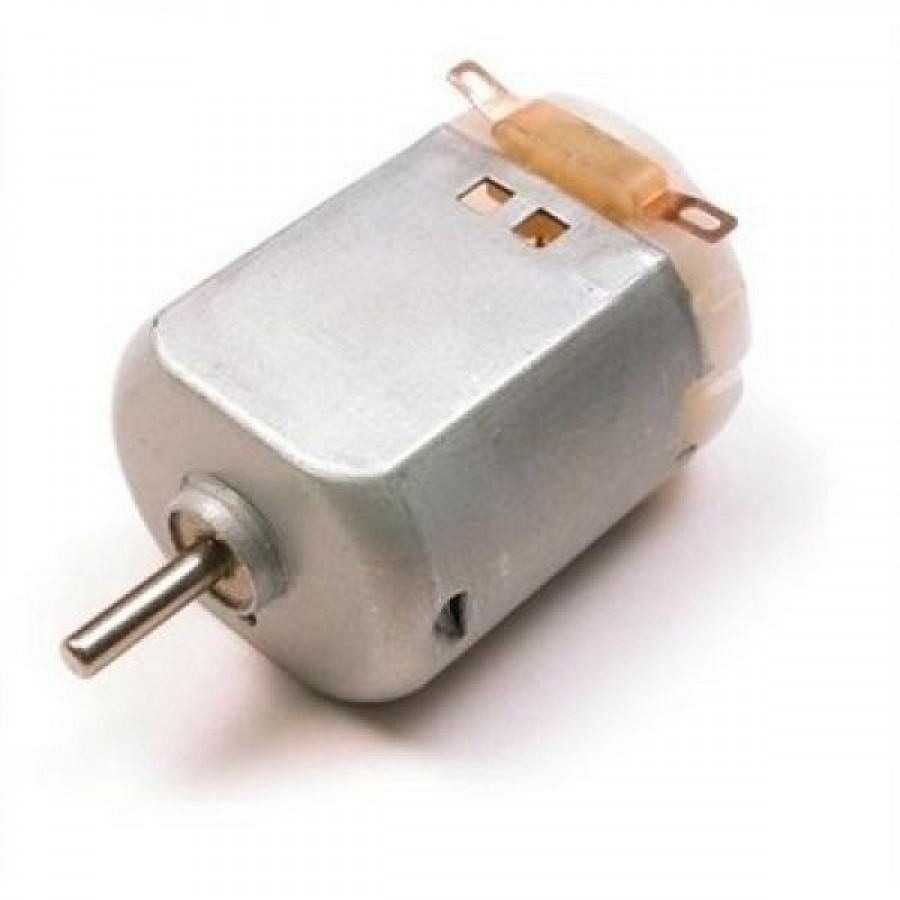
\includegraphics[width = 0.3\linewidth]{figures/brushed.jpg} &
   				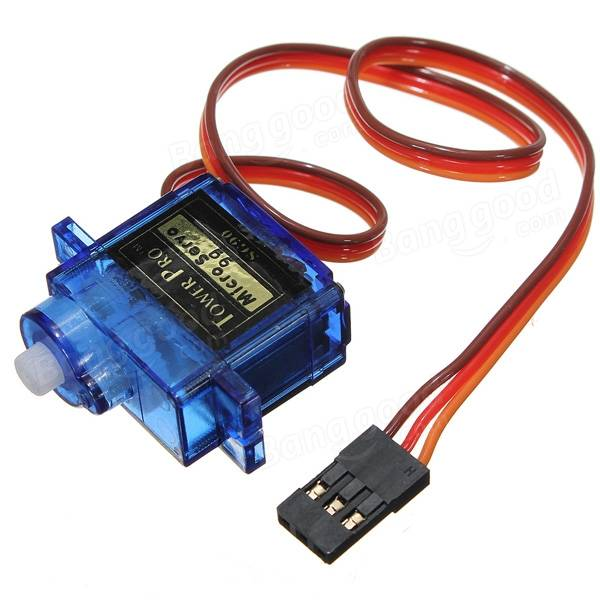
\includegraphics[width = 0.3\linewidth]{figures/stepper.JPG} & 
   				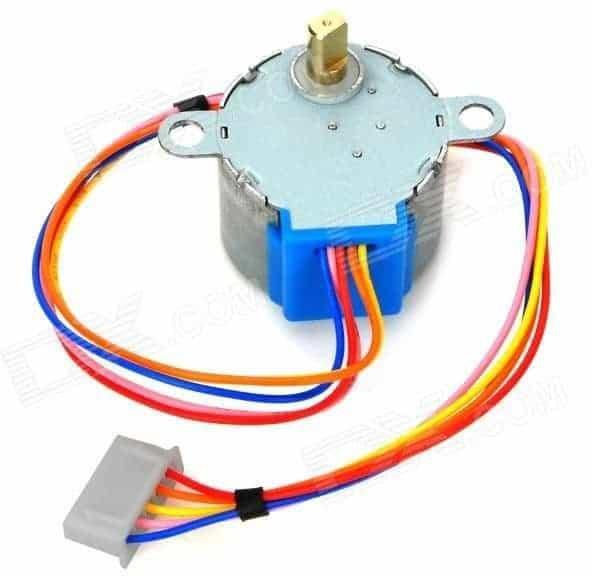
\includegraphics[width = 0.3\linewidth]{figures/paso.jpg}
   			\end{tabular}
   		\end{figure}
   		
   		\begin{itemize}
   			\item \textbf{Motores de escobillas}
   			\item \textbf{Servo motores} 
   			\item \textbf{Motores de paso}
   		\end{itemize}
    \end{frame}
    
    \begin{frame}
    	\begin{itemize}
    		\item Protocolo UART
    		\begin{figure}[h]
    			\centering
    			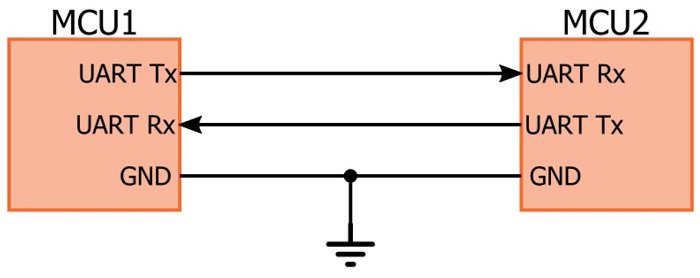
\includegraphics[width = 0.5\linewidth]{figures/uart.jpg}
    		\end{figure}
    		\item Microcontrolador
    		\begin{figure}[h]
    			\centering
    			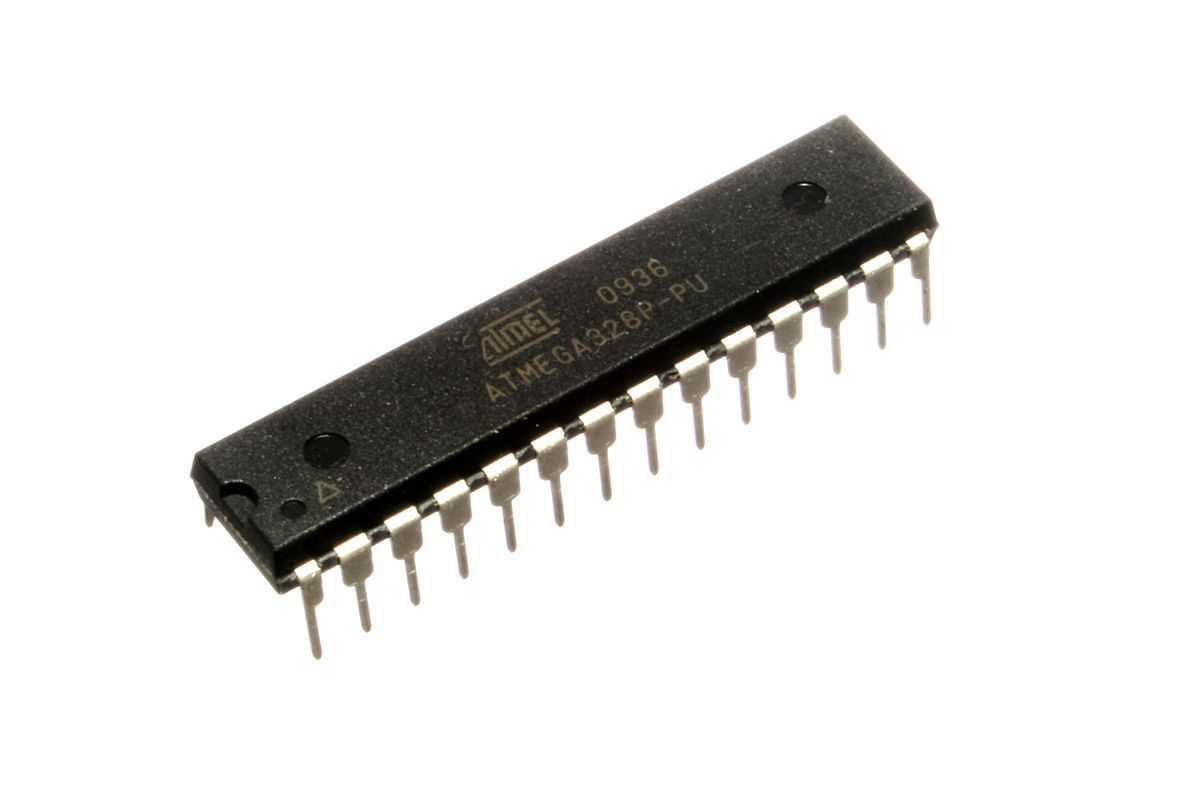
\includegraphics[width = 0.5\linewidth]{figures/atmega.jpg}
    		\end{figure}
    	\end{itemize}    
    \end{frame}
    
    \section{Fabricación y resultados}
    \begin{frame}{Fabricación y resultados}
    	Tres modelos fueron diseñados, solo dos fueron probados.
    	\begin{figure}
    		\centering
    		\begin{tabular}{ccc}
   				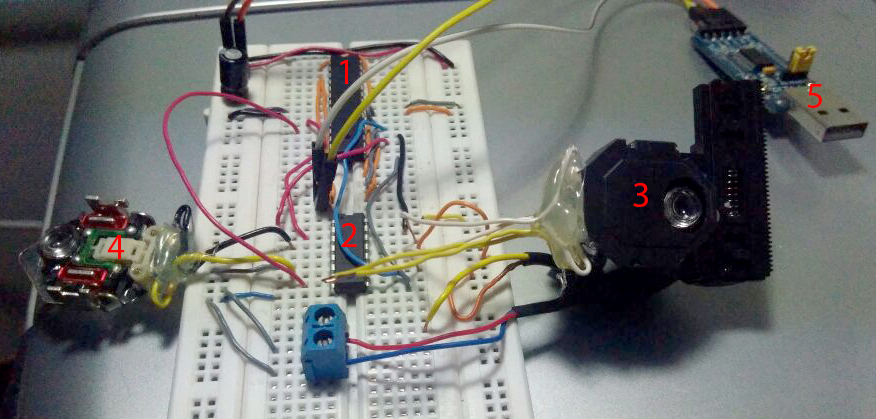
\includegraphics[width=0.3\linewidth]{figures/breadboard} & 
   				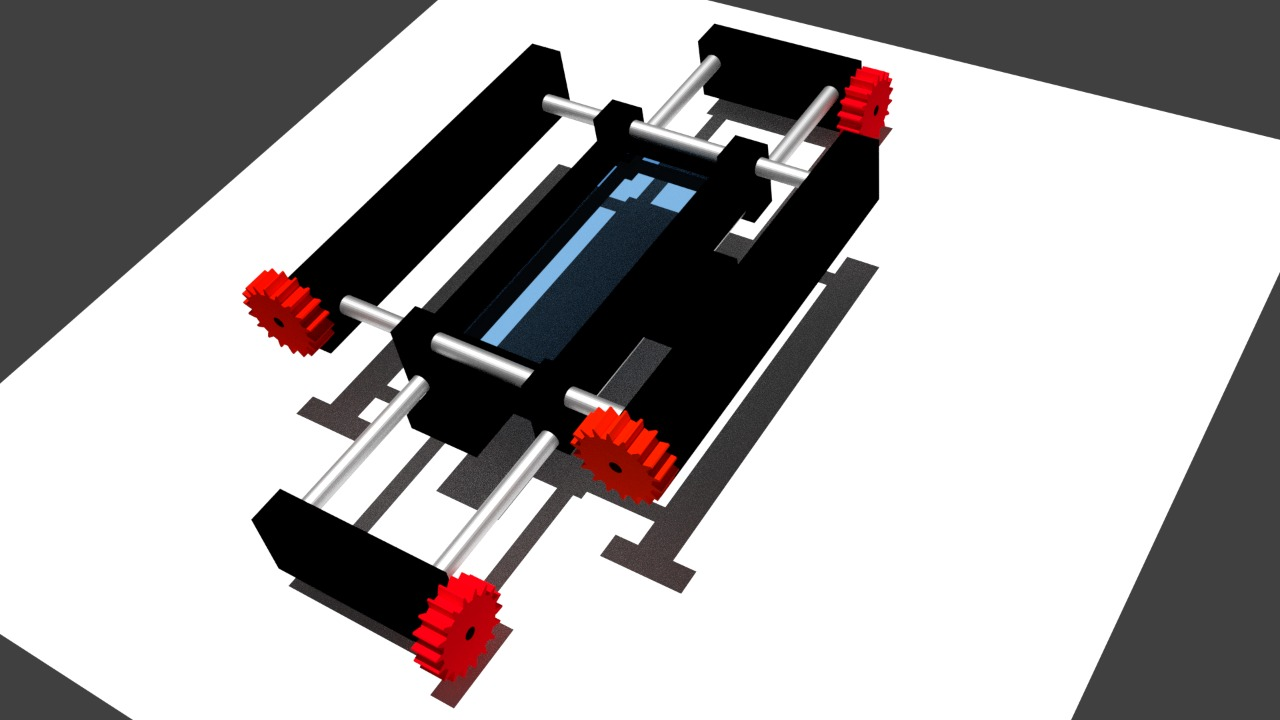
\includegraphics[width=0.3\linewidth]{figures/system2.jpg} &
   				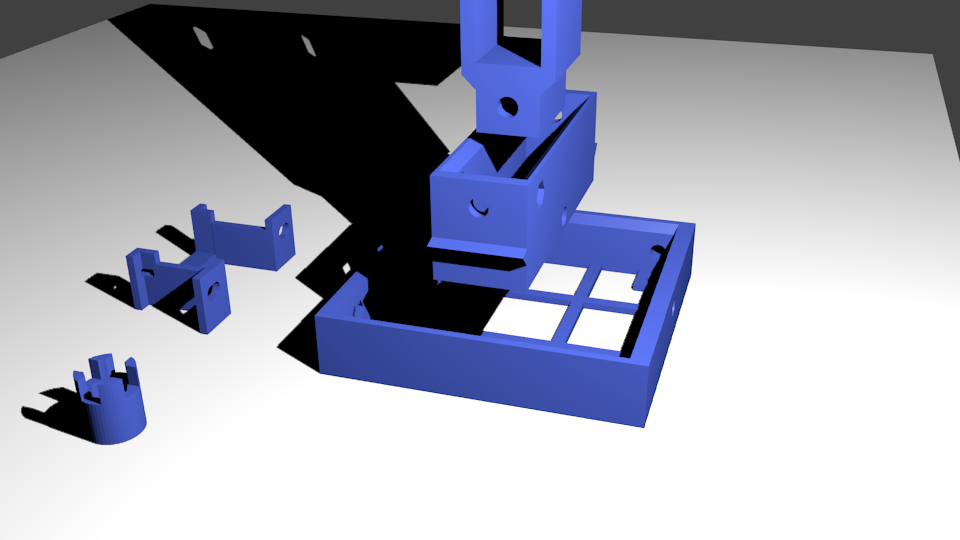
\includegraphics[width=0.3\linewidth]{figures/model3.png}
    		\end{tabular}
    	\end{figure}
    \end{frame}
    
    \subsection{Modelo 1}
    \begin{frame}{Modelo 1}
    	Construído a partir de un sistema de lectura de CD.
    	\begin{columns}
    		\column{0.45\textwidth}
	    		\begin{figure}[h]
	    			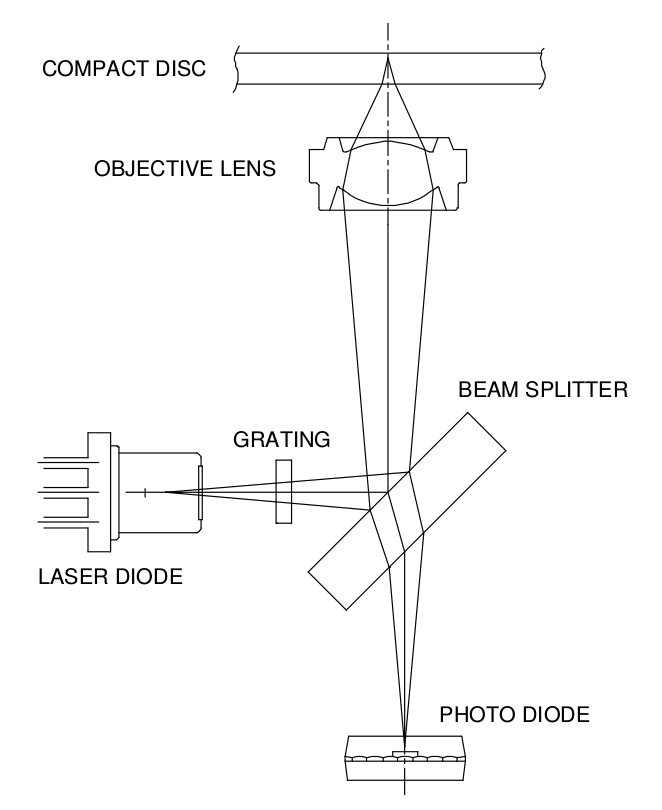
\includegraphics[width=0.9\linewidth]{figures/cdsystem.png}
	    		\end{figure}
	    	\column{0.45\textwidth}
		    	\begin{figure}
		    	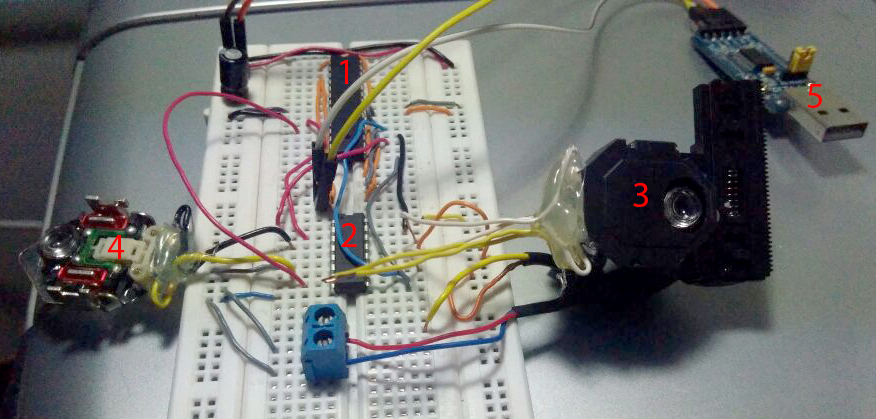
\includegraphics[width=0.9\linewidth]{figures/breadboard}
		    	\end{figure}
    	\end{columns}
    \end{frame}
    \begin{frame}{Modelo 1}
    	\begin{figure}[h]
    		\centering
    		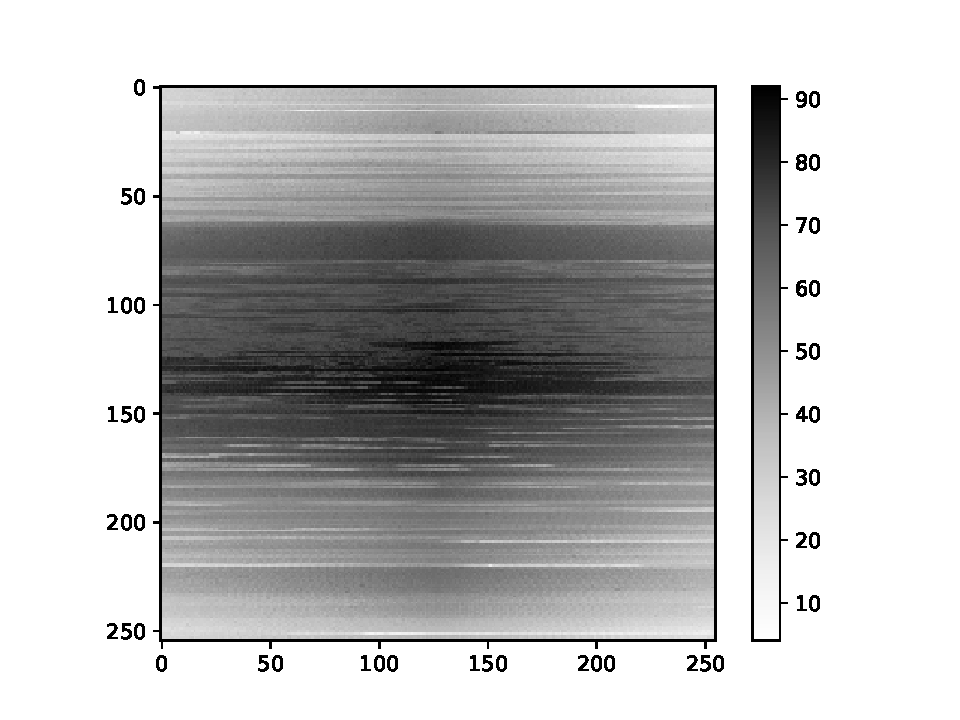
\includegraphics[width=0.62\linewidth]{figures/complete.pdf}
    	\end{figure}
    	Resultados obtenidos usando el primer stage. Se observa la primera línea horizontal de la letra E impresa sobre papel.
    \end{frame}
    
	\subsection{Modelo 2}
    \begin{frame}{Modelo 2}
    	Aislamiento de los motores al sistema usando correas de transporte.
        \begin{figure}[h]
        	\centering
        	\begin{tabular}{cc}
        		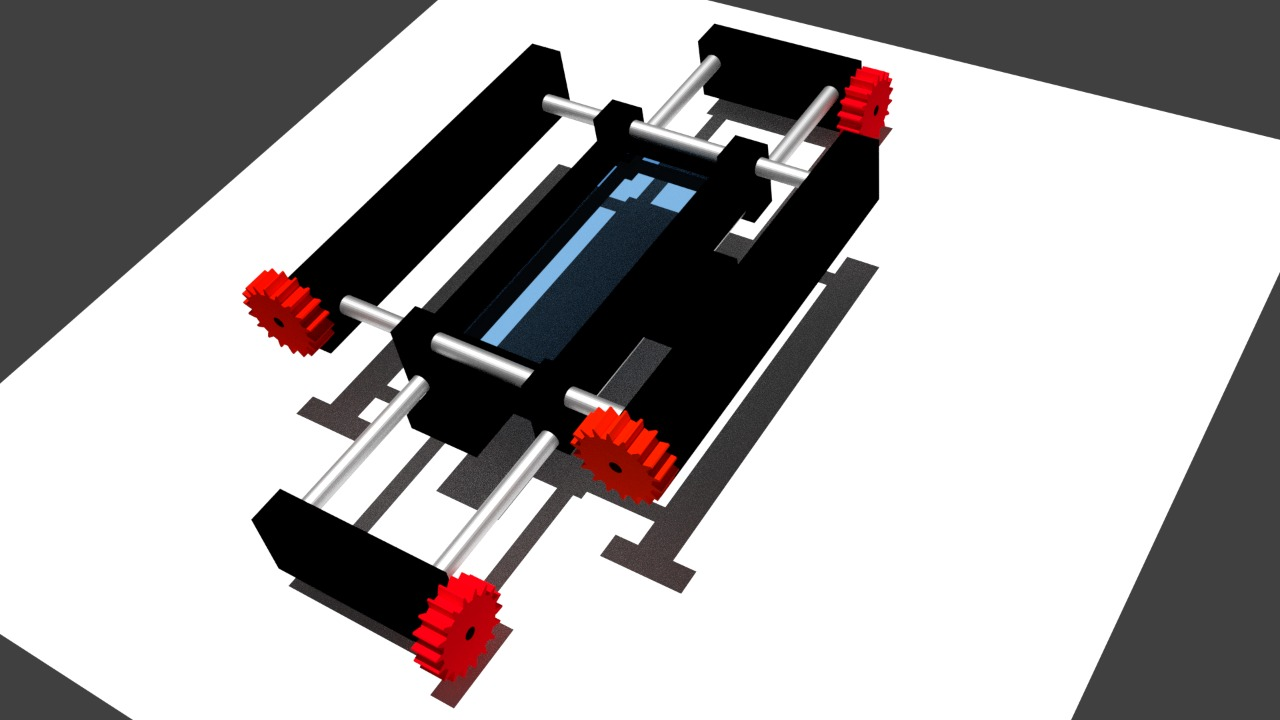
\includegraphics[width=0.45\linewidth]{figures/system2.jpg} & 
        		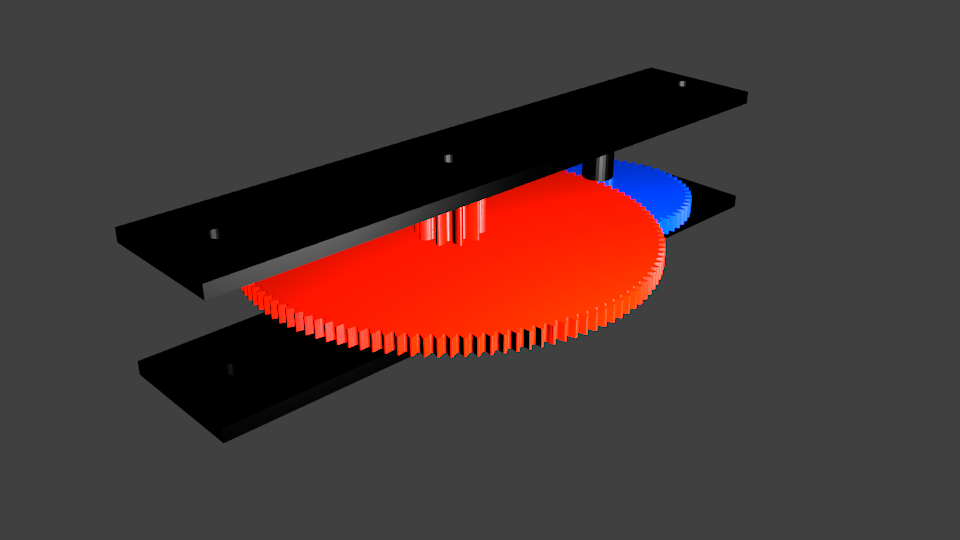
\includegraphics[width=0.45\linewidth]{figures/model2.png}
        	\end{tabular}
        \end{figure}
        Se requiere un motoreductor.
    \end{frame}
    
    \subsection{Modelo 3}
    \begin{frame}{Modelo 3}
        \begin{figure}[h]
        	\centering
        	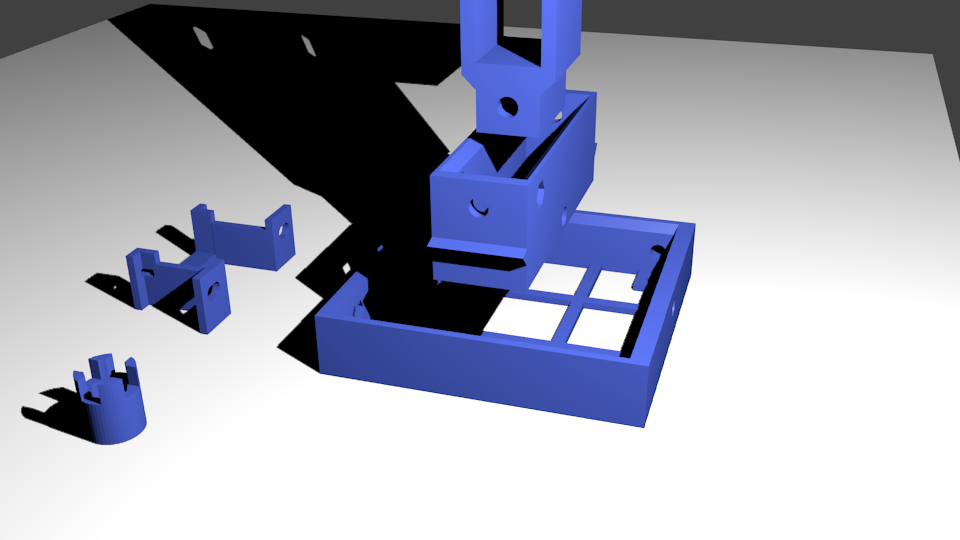
\includegraphics[width=0.5\linewidth]{figures/model3.png}
        \end{figure}
        
        Además de las piezas de impresión, también fue necesario adquirir:
        \begin{itemize}
        	\item 12 Tornillos M3 de 10 mm.
        	\item 2 Tornillos 15/32" de 100 mm.
        	\item 1 Tornillo 15/32" de 50 mm.
        	\item 12 Tuercas M3.
        	\item 6 Tuercas 15/32".
        \end{itemize}
    \end{frame}
    
    \begin{frame}{Modelo 3}
    	Distancia disponible de movimiento en cada dirección del stage
    	\begin{table}[h]
    		\centering
    		\begin{tabular}{cc}
    			\hline
    			\textbf{Eje} & \textbf{Distancia (cm)} \\
    			\hline
    			$x$ & $3.42 \pm 0.01$ \\
    			$y$ & $3.90 \pm 0.01$ \\
    			$z$ & $1.31 \pm 0.01$ \\
    			\hline		
    		\end{tabular}
    	\end{table}
    	El movimiento de los motores se lleva a cabo por el microcontrolador quien recibe información del computador usando protocolo UART.
    \end{frame}
    
    \begin{frame}{Modelo 3}
    	Movimiento mínimo en cara dirección:
   		\begin{table}[h]
   			\centering
   			\tiny
   			\begin{tabular}{cc}
   				\hline
   				\textbf{Eje} & \textbf{Distancia ($\mu$m)} \\
   				\hline
   				$x$ & $1.55$ \\
   				$y$ & $1.49$ \\
   				$z$ & $1.60$ \\
   				\hline		
   			\end{tabular}
   		\end{table}
    	
    	Variación y rapidez en función de la resolución para el eje $x$ y $y$, correspondientemente.
    	\begin{figure}[h]
    		\centering
    		\begin{tabular}{cc}
    			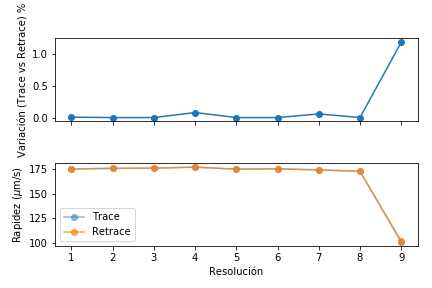
\includegraphics[width=0.45\linewidth]{figures/x.png} & 
    			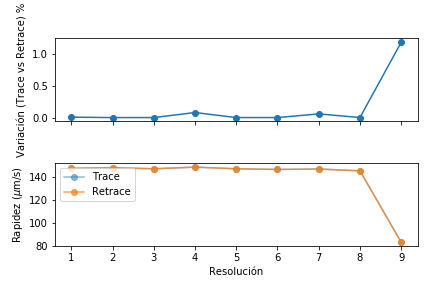
\includegraphics[width=0.45\linewidth]{figures/y.png}
    		\end{tabular}
    	\end{figure}  	
    \end{frame}
    \begin{frame}{Modelo 3}
    	Optimización del enfoque con la construcción de un plano.
    	\begin{figure}[h]
    		\centering
    		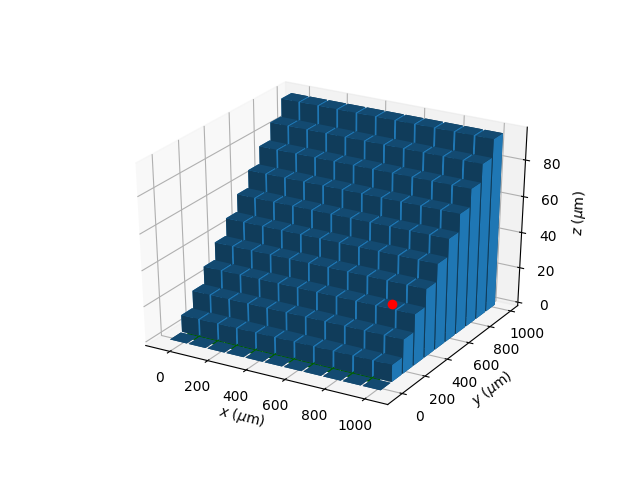
\includegraphics[width=0.7\linewidth]{figures/plane.png}
    	\end{figure}
    \end{frame}
    
    \section{Conclusiones}
    \begin{frame}{Conclusiones}
        \begin{itemize}
        	\item Tres modelos distintos fueron propuestos.
        	\item Obtención de una imagen de 7 bits.
        	\item Implementación de la librería Mauscope, escrita en Python.
        	\item Resolución de movimientos de hasta 1.49 $\mu$m. 
        	\item Velocidades de 73 $\mu$m/s hasta 176 $\mu$m/s.
        \end{itemize}
    \end{frame}
    
    \nocite{*}
    \begin{frame}{Referencias}
        \printbibliography
    \end{frame}
\end{document}